\documentclass[a4paper, 12pt, twocolumn]{article}
\usepackage{xeCJK}
\usepackage{amsfonts}
\usepackage{amsbsy}
\usepackage{amsmath}
\usepackage{enumitem}
\usepackage{indentfirst}
\usepackage{hyperref}
\usepackage{graphics}
\usepackage{graphicx}
\usepackage{booktabs}
\setlength{\parindent}{24pt}
\renewcommand{\abstractname}{摘要}
\renewcommand{\refname}{参考文献}
\renewcommand{\figurename}{图}
\renewcommand{\tablename}{表}
\newcommand{\figref}[1]{图~\ref{#1}}
% \newcommand{\eqref}[1]{公式\ref{#1}}
\title{综述:神经网络语言模型(译)}
\author{Zhipeng Zou}
\begin{document}
  \maketitle
  \begin{abstract}
    作为自然语言处理(Natural Language Processing,NLP)系统的核心组件,语言模型(Language Model,LM)能够提供词的向量表示和词序列的联合概率。神经网络语言模型(Neural Network Language Models,NNLM)克服了维度灾难,并且大大提升了传统语言模型的性能。本文主要阐述了神经网络语言模型综述。首先,本文大致描述了经典的神经网络语言模型结构,然后介绍和分析一些主流的模型改进方法。本文总结和对比了神经网络所用的数据集、工业实践中的一些工具库,以及一些神经网络语言模型研究方向。
  \end{abstract}
  \section{绪论}
  语言模型是大部分NLP任务的基础,如在机器翻译(Machine Translation,MT)任务中,语言模型被用来评估翻译系统输出一个特定序列的概率,以提升其在目标语言中的流畅度。而在语音识别(Speech Recognition,SR)任务中,将联合语言模型和声学模型来预测输出下一个词。

  早期的NLP系统主要基于人工编写的规则,该过程不仅耗时长,而且难以完成以至无法覆盖到多样的语言环境。20世纪80年代,人们提出了对于构成序列$s$的$N$个词的出现概率语言模型,即
  \begin{equation}
    \begin{aligned}
      P(s)&=P(w_1w_2\cdots w_N) \\
      &= P(w_1)P(w_2|w_1)\cdots P(w_N|w_1,\cdots,w_{N-1}),
    \end{aligned}
    \label{eq:1}
  \end{equation}
  其中$w_i$表示序列$s$中的第$i$个词,则给定一个词的前序序列(通常称为历史上下文或上下文),整个词序列的概率可分解为,下一个词关于其前向词的条件概率的乘积。

  考虑到难以学习上述模型中的大量参数,通常需要一种近似方法来近似表示。N元模型便是一种近似方法,并且在神经网络语言模型之前,一直作为最优模型而被广泛使用。$(k+1)$元模型都是基于$k$阶马尔可夫假设得来,该假设认为当前状态仅依赖于其之前的$k$个状态,并使用最大似然进行估计得出模型参数,即:
  \begin{equation}
    P(w_1|w_1\cdots w_{t-1}) \simeq P(w_k|w_{t-k}\cdots w_{t-1}),
    \label{eq:2}
  \end{equation}

  困惑度(Perplexity,PPL)\cite{jelinek1977perplexity}是一种语言模型评估方法,其本质上是一个信息论中概率模型质量评估指标。当困惑度值越低时,则表明模型更优。给定一个包含$N$个词的语料库和一个语言模型,则语言模型的困惑度被定义为:
  \begin{equation}
    2^{-\frac{1}{N}\sum_{t=1}^{N}\log_2 LM(w_t|w1\cdots w_{t-1})}.
    \label{eq:3}
  \end{equation}
  上述公式表明,困惑度与语料库紧密相关,因而两个或多个语言模型只有构建在相同的语料库上才能使用困惑度进行对比。

  然而,$n$元模型有个显著的特点,对于未在训练语料库出现的词,其序列的困惑度值为0,这与实际情况不符。而使用平滑技术能解决该问题,其主要思想是“劫富济贫”,即降低出现在训练语料库中的事件的概率,并将概率分配给未出现的事件。

虽然使用平滑技术的n元模型能够正常工作,却仍然有其他问题,其中维度灾难便是一个重大问题,从而大大制约了通用语言模型在大规模语料库上的建模能力,当人们想要对离散空间中的联合分布建模时,这个问题及其显著。例如,当你想要建模一个10,000词汇的$n$元语言模型时,便需要$10000^n-1$个参数。

为了解决这个问题,便引入了神经网络(Neural Network,NN)使语言模型映射到一个连续空间。包括前馈神经网络(Forward Feedback Neural Network,FFNN)和循环神经网络(Recurrent Neural Network,RNN)在内的神经网络都能自动学习到特征和连续的表征。因此,人们都希望神经网络能够应用于语言模型,甚至是其他的NLP任务,以适配自然语言的离散、组合和稀疏的特性。

第一个前馈神经网络语言模型( FFNN Language Model,FFNNLM)是由\cite{bengio2003neural}提出,通过学习词的分布式表示来解决维度灾难,使得一个词能够使用一个低维向量(称之为embedding)表示。FFNNLM比$n$元模型的性能更好。之后,循环神经网络语言模型(RNN Language Model,RNNLM)\cite{mikolov2010recurrent}也相继提出。从此以后,NNLM开始逐渐称为LM的主流技术,并且被迅速地开发出来。紧接着,长短期记忆循环神经网络语言模型(Long Short-term Memory RNN Language Model,LSTM-RNNLM)\cite{sundermeyer2012lstm}用于解决长期依赖问题。于此同时,大量的改进技术也相继被提出来,用于降低训练和验证时的损失以及PPL指标,如层次Softmax(Hierarchical Softmax),缓存机制等。近期,注意力机制在NNLM上的应用,使得模型的表现大幅提升。

本文主要集中于讨论NNLM的各种方法及其发展趋势。在第\ref{sec:classic-NNLM}节我们将介绍经典神经网络语言模型,第\ref{sec:3}节将分别讨论和分析NNLM的各类改进方法,紧接着,在第\ref{sec:4}和\ref{sec:5}节将介绍常用的数据集和工具库,最后,得出本文的结论,并讨论今后NNLM的研究方向。

\begin{figure}[!htp]
  \centering
  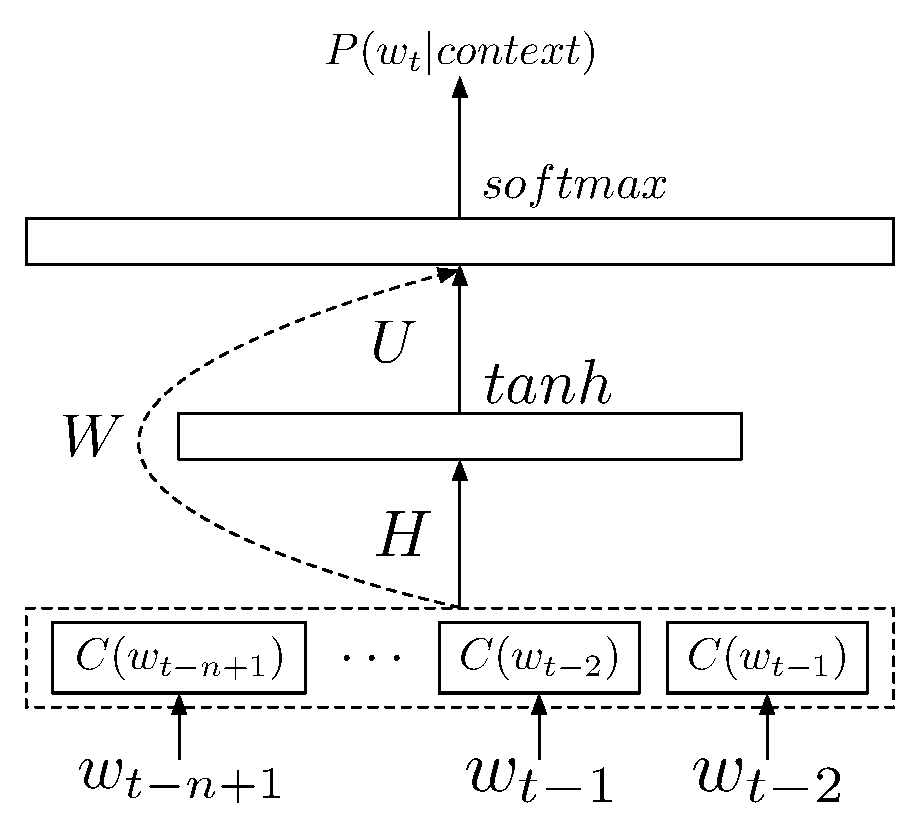
\includegraphics[width=\columnwidth]{figure-1.eps}
  \label{figure:1}
  \caption{\cite{bengio2003neural}提出的FFNNLM,在这个模型中,为了预测$w_t$的条件概率,它前$t-1$个词根据索引被共享投影矩阵$C \in \mathbb{R}^{|V|\times m}$投影到一个连续的特征向量空间,其中$|V|$表示词库大小,$m$是特征向量的维度,即词$w_i$被投影为一个分布式特征向量$C(w_i)\in \mathbb{R}^m$。投影矩阵$C$是词库中每个词的特征向量。FFNN的输入$x$是有$n-1$个词的特征向量拼接而成。整个模型使用一个$Softmax$输出层保证输出词的条件概率为正并且和为1. 模型的学习算法是使用反向传播(backpropagation,BP)的随机梯度下降(Stochastic Gradient Descent,SGD)法。}
\end{figure}
\section{经典神经网络语言模型}\label{sec:classic-NNLM}
\subsection{前馈神经网络语言模型}
\cite{xu2000can}曾尝试将NN应用于LM,虽然他们的模型比基准的$n$元模型表现更优,但是由于没有隐藏层,其泛化能力太差而导致无法捕获到相关的特征。

根据公式\eqref{eq:1}的表示,LM的目标等价于评估一个条件概率$P(w_k|w_1\cdots w_{k-1})$,但是FFNN无法直接处理变长数据和高效地表示历史上下文,因而诸如LM的序列建模任务,FFNN都必须要求他们使用固定的长度作为输入。受$n$元语言模型的启发(见公式\eqref{eq:2}),FFNNLM会将前$n-1$个词作为预测下一个词的上下文。

\cite{bengio2003quick}提出了如\figref{figure:1}所示的最原始的FFNNLM结构,其能够表示为:
\begin{equation}
  y=b+Wx+U tanh(d+Hx)
  \label{eq:4}
\end{equation}
其中,$H,W,U$是用于连接各层的权重矩阵,$d,b$则分别是隐藏层和输出层的偏置值。

FFNNLM通过学习到每个词的分布式表示,来实现在连续空间上的建模。其中,词的表示只是LM用于提升其他NLP任务的副产品。基于FFNNLM,\cite{mikolov2013efficient}提出了两个表示模型:CBOW和Skip-gram。FFNNLM通过将词映射到低维向量,从而解决了维度灾难,并使得FFNN主导了NNLM的研究。

但是,这种方式仍然有缺点,在训练之前上下文的具体大小都受到限制,这和人们理解大量上下文然后作出推测的实际情况完全不符。序列中的词是具有时序特性的,而FFNNLM在建模时却无法利用。此外,相比于$n$元模型,虽然全连接神经网络减少了参数,但还是有大量需学习的参数,这仍然是高代价、低效率。

\begin{figure}[!htp]
  \centering
  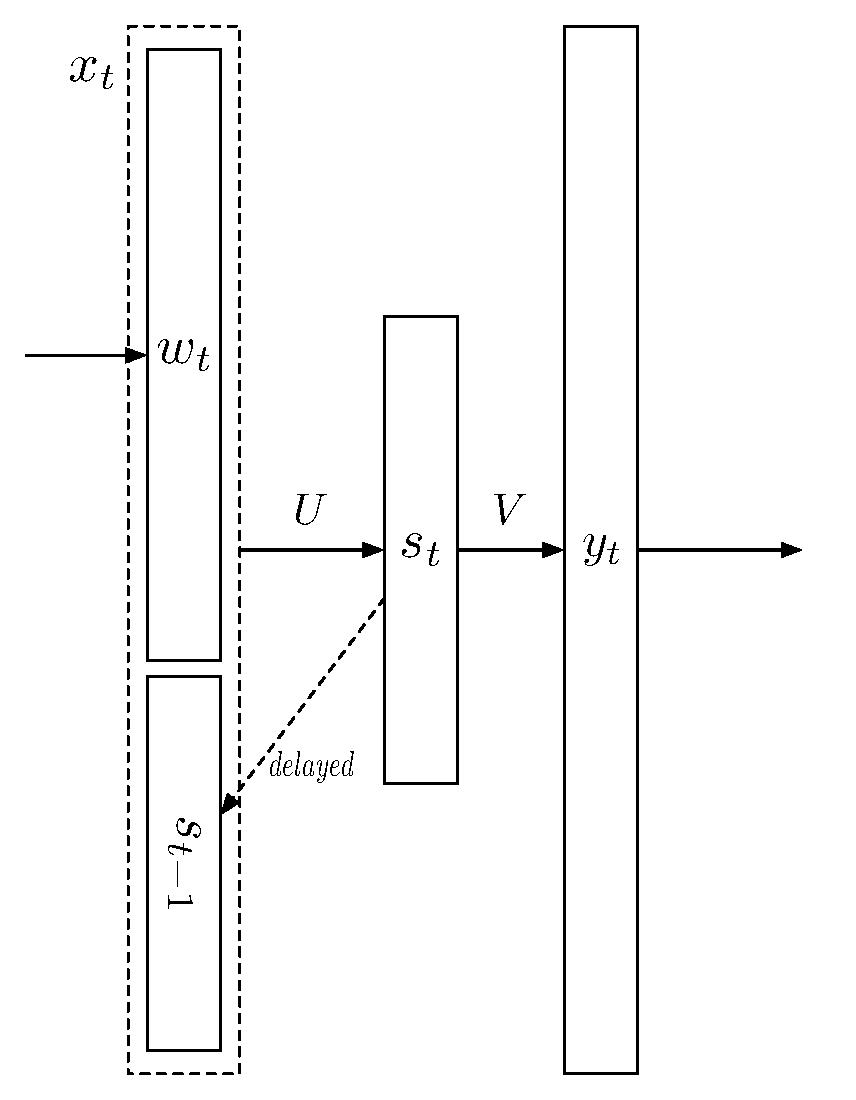
\includegraphics[width=.8\columnwidth]{figure-2.eps}
  \label{figure:2}
  \caption{\cite{mikolov2010recurrent,mikolov2011rnnlm}提出的RNNLM,RNN有一个随每个时间步输入而改变的内部状态,将内部状态叠加便可产生之前的上下文。状态$s_t$能够根据输入词$w_t$和上一个内部状态$s_{t-1}$获得。}
\end{figure}
\subsection{循环神经网络语言模型}
\cite{bengio2003neural}提出了RNN语言模型的思想,他们认为,将更多共享的结构和参数引入到NN中可以捕获更长的上下文信息。

首次提出RNNLM的是\cite{mikolov2010recurrent,mikolov2011rnnlm},如\figref{figure:2}所示,在每个时间步$t$,RNNLM都能表示为:
\begin{equation}
  \begin{aligned}
    x_t &= \left[w_t^\top ; x_{t-1}^\top \right]^\top , \\ 
    s_t &= f(Ux_t+b), \\ 
    y_t &= g(Vs_t + d),
  \end{aligned}
\end{equation}
其中$U,W,V$都是权重矩阵,$b, d$是隐藏层和输出层的偏置值。在\cite{mikolov2010recurrent,mikolov2011rnnlm}中,$f$是$sigmoid$函数,而$g$是$softmax$函数。RNNLM可以通过BPTT或截断的BPTT算法进行训练。实验显示,RNNLM比FFNNLM和$n$元模型在PPL指标上都更优。

相较于FFNNLM,RNNLM取得了技术突破,因为RNN在处理序列数据时具有先天优势,其可以接受任何变长的输入。移动输入窗口时,由于RNN的内部状态机制从而避免了重复的计算。并且,在时间$t$由输入引起的内部状态变化,便揭示了这类时序信息,而RNN中的参数共享又进一步地减少了模型参数量。

尽管RNNLM可以利用所有上下文进行预测,但是在训练时,模型很难做到长期依赖。因为RNN训练期间可能产生梯度消失或爆炸,从而使得训练速度变慢或参数值无穷大。

\subsection{长短期记忆的循环神经网络语言模型}
长短期记忆(LSTM)RNN解决了上述长期依赖的问题,因此,\cite{sundermeyer2012lstm}将LSTM引入到了LM中,提出 LSTM-RNNLM。除了记忆单元和神经元网络的结构,LSTM-RNNLM的框架几乎与RNNLM完全相同。 在LSTM记忆单元中,添加了三个门结构(包括输入,输出和遗忘门),以控制信息流。 LSTM-RNNLM的一般结构可以表示为:
\begin{equation}
  \begin{aligned}
    f_t &= \sigma(U_t x_t + W_t h_{t-1} + b_t)\\ 
    i_t &= \sigma(U_i x_t + W_i h_{t-1} + b_i)\\ 
    o_t &= \sigma(U_o x_t + W_o h_{t-1} + b_o)\\ 
    \widetilde{C}_t &= f\left(U_x x + W_x h_{t-1} + b_x\right) \\
    C_t &= f_t \odot C_{t-1} + i_t \odot \widetilde{C}_t \\
    h_t &= f(C_t) * o_t \\
    y_t &= f(U_y x_t + W_y h_t + b_y) \\
  \end{aligned}
\end{equation}
其中,$f$表示$tanh$函数,$\sigma$为$sigmoid$函数,$f_t, i_t, o_t$表示遗忘门,输入门,输出门,$U_t, U_i, U_o, W_t, W_i, W_o$表示各门的参数,$U_x, W_x, b_x$表示细胞状态更新的参数,$C_t$表示$t$时刻的细胞状态,$U_y, W_y, b_y$表示输出层的参数。(这里的翻译、公式和原文不同)

对比上述三种经典语言模型,RNNLM(包括LSTM-RNNLM)比FFNNLM表现更好,并且LSTM-RNNLM为最优的LM,而当前的NNLM也大多基于RNN或LSTM。

纵使LSTM-RNNLM效果很好,但是在大规模语料库训练该模型仍然很耗时间,因为预测目标词的概率分布是通过$softmax$层进行归一化,但$softmax$在计算对数似然时,需要考虑整个词库中的词。
所以,人们都希望能有更高效的语言模型。为了改进NNLM,研究者们仍在持续探索各种契合人类处理自然语言习惯的技术。
\section{改良技术}\label{sec:3}
\subsection{降低困惑度的技术}
为了降低困惑度,各种新的结构、有效信息都被引入到经典NNLM中,如LSTM-RNNLM。受语言学和人类处理自然语言习惯的启发,人们相继提出了一些新颖而又有效的方法,如字符感知模型,因子模型,双向模型,缓存和注意力机制等。

\paragraph{字符感知模型} 在自然语言中,形似词通常也义似,如\textit{superman}和\textit{policeman}中的\textit{man}具有相同的意义。
\cite{mikolov2012subword}也在字符级进一步研究了RNNLM 和 FFNNLM,事实证明,字符级的NNLM能够用于解决未知词(out-of-vocabulary,OOV)问题。由于字符特征揭示了词语间的结构相似性,从而提升了模型对罕见词和未知词的建模能力。
由于字符级NNLM在$Softmax$层的小规模输出,使所需训练的参数数量大大减少。但是,实验结果显示,训练得到高精度的字符级NNLM很艰难,因为字符级NNLM必须考虑更长的上下文,才能正确地预测下一个词。

很多的解决方案提出,要将字符级和词级信息进行组合,并称其为字符感知LM。其中一种方法便是,先逐词提取字符级特征,然后在将其应用至词级LM。\cite{kim2016character}提出使用卷积神经网络(Convolutional Neural Network, CNN)来抽取字符级特征,然后使用LSTM在每个时间步来处理这些词的字符级特征。同时,[Hwang and Sung, 2016]使用了由多个具有不同时间登记的模块组成的分层RNN结构解决了字符级NNLM问题。另有一种解决方案是将字符级和词级特征一同输入到NNLM中,\cite{miyamoto2016gated}认为可以用双向LSTM从词中提取的字符级特征向量对词特征向量进行插值,然后将该向量作为LSTM的输入。\cite{verwimp2017character}提出了一个字符-词的LSTM-RNNLM方法:将字符级特征向量和词级向量拼接,再将拼接后的向量输入到后续网络。字符感知语言模型直接使用字符级LM作为词级LM的字符特征提取器,从而使得LM能够使用字符级和词级特征来进行预测。

\paragraph{因子模型}
NNLM基于符号标记来定义单词的相似性,但是,它同时也可以从词型特征(词缀,大小写,连字符等)或其他标注(例如词性)特征中得出。受到因子LM的启发,\cite{alexandrescu2006factored}提出了一种新型的神经概率LM:因子分解NNLM,来学习词和词的特定特征到连续空间的映射。

许多研究都探讨过因子的选择问题,但首先需要考虑的是不同的语言特征。 \cite{wu2012factored}引入了词形,语法和语义特征来扩展RNNLM。 \cite{adel2015syntactic}在其他因子上也付诸探索,例如词性标注,布朗词簇,开放类词和开放类词嵌入簇。实验结果表明,布朗词簇,词性标签和开放词特征是普通话-英语转换任务中最有效的几类特征。此外,人们还探讨了上下文信息。例如,\cite{mikolov2012subword}从固定长度块中的前词序列,计算出其主题分布。 \cite{wang2015larger}提出了一种将语料词袋(BoW)上下文整合到语言模型中的新方法。此外,文本无关因子的方法也陆续提出。\cite{ahn2016neural}提出了一种神经知识语言模型,将知识图谱符号知识应用于RNNLM。

因子模型能够使用某些相同特征,来归纳单词类别。将词符号以外的因子应用于神经网络训练,可以更好地学习词的连续表示,OOV词,并降低LM的PPL。但是,不同的因子选择取决于LM不同的上游NLP任务、应用程序等。只能分别尝试各种因子,才可加以选择。因此,对于特定任务,必须有一种有效的因子选择方法。同时,必须建立带有因子标签的语料库。
\paragraph{双向模型}
传统的单向神经网络单纯地从输入预测输出概率,而双向神经网络的建立则还会考虑未来数据的条件。\cite{graves2013hybrid,bahdanau2014neural}则将双向RNN和LSTM神经网络(即BiRNN和BiLSTM)引入到了语音识别等其他NLP任务。双向RNN通过从两个方向处理输入数据,从而能够利用过去和未来的上下文信息。其中,最热门的双向模型的工作便是ELMo模型\cite{peters2018deep},即一种全新的基于BiLSTM-RNNLM的深度上下文词表示方法。预训练ELMo模型嵌入层的向量,便是词库中所有词学习到的向量表示。将这些表示作为嵌入层加入到现有模型后,这些模型在6个困难的NLP任务中都取的了最优效果。

尽管使用过去和未来上下文的双向语言模型能够有显著提升,但BiLM不能直接用于语言模型,因为语言模型定义是历史上下文。由于在机器翻译、语音识别的NLP任务中,单词序列被视为一次性的输入序列,因此双向语言模型能适用于上述任务。
\paragraph{缓存机制}
"最近出现的单词可能会再次出现",基于这个假设,最初人们使用缓存机制来优化$n$元语言模型,从而突破了依赖项的长度限制。该方法,会在缓存的历史记录中匹配新输入。缓存机制最初是用来降低NNLM的PPL。\cite{soutner2012neural}尝试将FFNNLM与缓存机制结合,并提出了基于缓存的NNLM的结构,但是这导致概率变化离散化。为了解决这个问题,\cite{grave2016improving}
提出了一个连续的缓存模型,使得概率变化依赖于隐藏层的内积。

另一种缓存机制是将缓存作为NNLM的加速技术,其主要思想是将语言模型的状态和输出存储于一个哈希表中,在给定相同的历史上下文时可快速得出预测结果。例如\cite{huang2014cache}使用4个缓存来加速模型的推理。这些缓存分别是对语言模型概率缓存的检索,对隐藏状态向量缓存的历史,对类别归一化因子缓存的历史以及对子词归一化因子缓存的历史和类别Id。

\paragraph{注意力机制}
RNNLM通过上下文来预测下一个词,但不是每个上下文的词都与下一个词相关或对预测下一个词有用。类似于人,带有注意力机制的语言模型会从较长的历史上下文中高效地选择有用词的表示,使得语言模型只会关注上下文中的某些特定词。\cite{bahdanau2014neural}率先提出注意力机制在NLP任务中的应用,\cite{tran2016recurrent,mei2017coherent}证明注意力机制能够有效地提升RNNLM的表现。

注意力机制通过注意力系数来获得目标域关于每个输入所需的关注程度,该注意力向量$z_t$通过符号$r_0,r_1,\cdots,r_{t-1}$的表示计算所得:
\begin{equation}
  z_t=\sum_{i=0}^{t-1}\alpha_{ti}r_{i\cdot}
  \label{eq:7}
\end{equation}
其中,$r_i$表示第$i$个词的表示,注意力系数$\alpha _{ti}$为$e_{ti}$经过$Softmax$函数归一化的值,而$e_{ti}$为:
\begin{equation}
  e_{ti}=a\left(h_{t-1}, r_i\right),
\end{equation}
表示一个对齐模型,用于评估符号$r_i$和隐藏状态$h_{t-1}$的匹配程度,该注意力向量是历史上下文很好的表示方法。

注意力机制被广泛应用于计算机视觉(Computer Vision,CV)和NLP领域,为此也提出了很多注意力的改进方法,这其中便包括软/硬注意力(soft/hard attention),全局/局部注意力(global/local attention),键-值/键-值预测注意力(key-value/key-value-predict attention),多维注意力(multi-dimensional attention),有向自注意力(directed self-attention),自注意力(self-attention),多头注意力(multi-head attention)等。这些注意力机制的改进版在语言模型中的使用都提升了语言模型的质量。

基于上述改进版注意力机制,又提出了各种强大的语言模型或词表示方法,如\cite{vaswani2017attention}提出的Transformer逐渐称为了后续开发的基础。Transformer是一个新颖的完全基于注意力机制的模型,其包含了编码和解码两部分。紧接着,\cite{radford2018improving}和\cite{devlin2018bert}分别提出GPT(Generative Pre-Training)和BERT(Bidirectional Encoder Representations from Transformers)模型,不同的是,GPT使用了Transformer的解码器,而BERT使用了编码器,并且BERT是一个双向注意力模型。不像CBOW, Skip-gram, and ELMo, GPT和BERT使用整个模型的全部参数来表示词向量,他们都是当前NLP中的最优词向量方法。由于注意力机制在诸多任务中的应用,慢慢成为了当前最热的研究方向。尽管目前已经有各种结构的注意力机制,但以注意力机制为核心的单词相似度方法表现仍不佳。因此,研究向量相似性的新方法是改善注意力机制的重要部分。


\subsection{大语料加速技术}
当前,在大量词汇的数据集上训练模型非常耗时,这主要是因为$Softmax$层都需要在整个词库上输出,所以现有很多方法都是为了解决神经网络训练中输出空间大的问题而提出。基本上,它们可以分为4类:层次$Softmax$法,采样近似法,自归一法以及精确梯度法,其中前两个方法使用最广。

\paragraph{层次 Softmax 法}
现在提出的一些基于分层$Softmax$的方法,会将目标条件概率分解为多个条件概率。\cite{morin2005hierarchical}便使用一个双向输出层二叉树(来自知网的相似性),使得预测的$V$个词变成了树的$V$个叶子节点。该方法可以使词的预测概率及其梯度计算量呈指数级下降。但是,尽管使用了专家知识,它的表现仍要比非层次方法差得多。\cite{mnih2009scalable}通过简单的特征法对其进行改进,从数据中自动构建词树。上述两个模型的表现很大程度上都取决于该启发式构建的树。

为解除二叉树的约束,\cite{le2012structured}引入了一个全新的,通用的,基于分类的,具有结构化输出层的NNLM,即结构化输出层NNLM。给定历史向量$h$和词$w_i$,条件概率可表示为:
\begin{equation}
  \begin{aligned}
    P(w_t|h) &=P(c_1(w_t)|h) \\ &\prod _{d=2}^D P(c_d(w_t)|h,c_1,\cdots,c_{d-1}).
  \end{aligned}
  \label{eq:9}
\end{equation}
此后,很多研究都改进了该模型,如基于词频分类层次模型和\cite{si2012impact}发布的布朗聚类层次模型,实验证明,该模型表现很好。\cite{zweig2013speed}提出一个速度优化分类方法,即一种动态编程算法,可通过最小化模型的运行时间来确定类别数。层次$Softmax$能在不增加PPL的情况下,显著减少模型参数量,这是因为该方法使用了$d+1$个$Softmax$层用于输出$^{d+1}\sqrt{|V|}$个类或者$\log_2 |V|$个二分类,而不是使用一个$|V|$个类的$Softmax$层。尽管如此,层次$Softmax$仍使得NNLM表现更差,但Brown clustering方法是一个特例。同时,已有的基于类别的方法,还是没有考虑上下文。现有的方法,分类还是硬分类,这是导致PPL增加的关键。因此,有必要研究一种基于软分类的方法,使得既能降低NNLM训练损失,又能使PPL保持不变,甚至降低。

\paragraph{采样近似法}
NNLM在计算下一个词的条件概率时,输出层使用$Softmax$会在损失计算量很大,并且归一化分母也很大。因此,有一种方法是随机或试探性地选择一小部分输出,从中估计概率和梯度。

受最小化对比散度的启发,\cite{bengio2008adaptive}提出了一个重要的采样方法和一个自适应的采样方法来加速NNLM的训练。其对数似然的梯度可被表示为:
\begin{equation}
  \begin{aligned}
    &\frac{\partial \log P(w_t|w_1^{t-1})}{\partial \theta} =-\frac{\partial y(w_t,w_1^{t-1})}{\partial \theta} \\ 
    & + \sum _{i=1}^k P(v_i|w_1^{t-1})\frac{\partial y(v_i, w_1^{t-1})}{\partial \theta}
  \end{aligned}
  \label{eq:10}
\end{equation}
负项的加权和是通过重要的样本估计获得的,即用$Q$代替$P$进行采样。因此,归一化分母和对数似然梯度的估计分别为:
\begin{equation}
  \hat{Z}\left(h_{t}\right)=\frac{1}{N} \sum_{w^{\prime}} \sum_{Q\left(\cdot | h_{t}\right)} \frac{e^{-y\left(w^{\prime}, h_{t}\right)}}{Q\left(w^{\prime} | h_{t}\right)}
  \label{eq:11}
\end{equation}
\begin{equation}
  \begin{aligned}
    &E\left[\frac{\partial \log P\left(w_{t} | w_{1}^{t-1}\right)}{\partial \theta}\right]=-\frac{\partial y\left(w_{t}, w_{1}^{t-1}\right)}{\partial \theta} 
\\ &+\frac{\sum_{w^{\prime} \in \Gamma} \frac{\partial y\left(w^{\prime}, w_{1}^{t-1}\right)}{\partial \theta} e^{-y\left(w^{\prime}, w_{1}^{t-1}\right) / Q\left(w^{\prime} | w_{1}^{t-1}\right)}}{e^{-y\left(w^{\prime}, w_{1}^{t-1}\right)} / Q\left(w^{\prime} | w_{1}^{t-1}\right)}
  \end{aligned}
  \label{eq:12}
\end{equation}
实验结果显示,采用采样会加速NNLM训练至原来10倍而不会显著增加PPL。\cite{bengio2008adaptive}提出一种使用自适应$n$元模型的自适应采样方法,而未使用\cite{bengio2003neural}中的1元模型。其他很多改进方法也有提出过,如并行训练小模型以估计采样损失,多重采样和似然加权方案,两步采样等。此外,还有其他不同的采样方法用于训练NNLM,包括噪声比较估计,局部敏感哈希(LSH)技术,BlackOut。

这些方法都利用采样方法显著提升了NNLM的训练,但是模型的评估计算量仍然很大。目前,基于采样近似法的模型计算复杂度仍然很高,但采样策略相对简单。除LSH方法外,人们都会随机地或启发式地选择其他的策略。

\begin{table}[t]
  \tiny
  \centering
  \caption{小数据集的大小(词数)}
  \begin{tabular}{lrrrr}
    \toprule \\ 
    Corpus & Train & Valid & Test & Vocab \\
    \midrule \\
    Brown & 800,000 & 200,000 & 181,041 & 47,578 \\ 
    Penn Treebank & 930,000 & 74,000 & 82,000 & 10,000 \\ 
    WikiText-2 &2000,000 & 220,000 & 250,000 & 33,000 \\ 
    \bottomrule
  \end{tabular}
  \label{table:1}
\end{table}
\section{数据集}\label{sec:4}
如上所述,有必要评估同一语料库上的所有LM,但这是不切实际的。 本节介绍一些常见的语料库。

通常,为了降低训练和测试时的损失,模型的可行性需先在小数据集上验证。公开的小数据集包括:Brown,Penn Treebank和WikiText-2,见表\ref{table:1}。

在模型结构确定之后,便需要在大规模数据集上训练和评估,来保证模型有足够的泛化能力。公共大规模数据集都会不定时通过其网站,新闻等方式更新,如Wall Street Journal, Wikipedia, News Commentary, News Crawl, Common Crawl, Associated Press (AP) News, 以及其他数据集。

然而,语言模型通常都是在不同的大规模数据集上训练。即使是在相同的数据集上,很多预处理方法和不同的训练集/验证集分割都会影响模型的结果。同时,训练时间的给定方式在各个文章中都不同,甚至是压根不提及。所以,不同文章的实验结果不能简单地拿来直接比较。
\section{工具库}\label{sec:5}
传统LM的工具库主要包含:CMU-Cambridge SLM, SRILM, IRSTLM, MITLM, BerkeleyLM,但是仅支持训练和评估$n$元语言模型和一系列的平滑技术。随着深度神经网络的发展,逐渐有很多基于NNLM的工具库问世。\cite{mikolov2010recurrent}发布了RNNLM工具库,支持训练和优化语音识别和机器翻译模型,但是不支持并行训练和GPU加速。\cite{schwenk2013cslm}构建了开源神经网络工具CSLM(Continuous Space Language Modeling,连续空间语言模型)支持训练和评估FFNN。可扩展的神经网络模型工具库TheanoLM\cite{enarvi2016theanolm},支持训练语言模型,以评估句子并生成文本。

根据我们的调查,没有任何工具能够同时支持传统$n$元模型和NNLM,并且它们一般不包含常用的语言模型的加载。
\section{未来展望}\label{sec:7}
大多数NNLM方法都是基于三种经典NNLM,而LSTM-RNNLM是目前最优的LM。一般有两大提升语言模型的方向:1)使用全新的结构或额外的知识来降低PPL;2)通过评估条件概率来加速模型训练和评估。

在调查过程中,我们发现并总结了一些NNLM的问题。因此,我们可以大致预估未来语言模型的发展方向。首先,降低损失和大量参数的方法仍然会被继续研究,以在保证PPL不增加的情况下加速模型训练和评估进程。其次,模拟人类工作方式的全新结构也是提升语言模型性能的重要方向。例如,构建一个通用模型也是今后的大方向,像GAN的方法。最后,但也值得一提的是,当前语言模型的评估方式都还不统一,因此有必要建立一个标准,来统一NLP的预处理过程,以及论文中模型的评估指标。
\section{结论}\label{sec:7}
NNLM的研究已经进行了近二十年,NNLM为NLP任务做出了很重要的贡献。本文研究了经典NNLM的不同框架及其改进方法,此外,还介绍了在NNLM研究中不可或缺的语料库和工具包。

  \bibliographystyle{plain}
  \bibliography{ref}
\end{document}